\documentclass[conference]{IEEEtran}
\input epsf
\usepackage{graphicx}
\usepackage[utf8]{inputenc}
\usepackage{url}
\usepackage[nolist]{acronym}
%\usepackage{biblatex}

\hyphenation{op-tical net-works semi-conduc-tor IEEEtran}
\begin{document}

\title{\LARGE BASA: Building Automation and Security on Android
}

\author{
  \IEEEauthorblockN{João Miguel Marques Sampaio\\
  joao.mm.sampaio@tecnico.ulisboa.pt}\\
  \IEEEauthorblockA{Instituto Superior Técnico, Universidade de Lisboa\\ 
  November 2016}
}


\maketitle

\begin{abstract}
Systems capable of reducing energy consumption are needed in order to reduce monetary energy costs for companies. At the same time, studies show that temperature can influence human productivity, thus simply removing \ac{HVAC} systems could impact negatively a company's employees work productivity.

Nowadays \ac{BAS} are used to manage a building, however traditional systems face a big problem, they have high monetary costs associated with installation and hardware. At the same time, the market is flooded with cheaper tablet devices with built-in sensors, connectivity and visual display.

In this document, we propose a system that utilizes an Android tablet, mounted in the room wall, running an application to achieve building automation. Our solution addresses the energy consumption problem, increases occupant comfort and offers security, including intrusion detection notification and video monitoring, to the user. The proposed system differs from traditional centralized \ac{BAS} by offering a distributed architecture with nodes deployed in every office and a user mobile application capable of interacting with the system.

\end{abstract}
% \IEEEoverridecommandlockouts
% \begin{keywords}
% Domain Registry, High availability, Load balancing, Monitoring, Registry Service, reThink H2020
% \end{keywords}

\IEEEpeerreviewmaketitle

\section{Introduction}
\label{introduction}

Buildings represent a large portion of the total energy consumed. According to the International Energy Agency, buildings represent 32\% of total final energy consumption~\cite{iea}. One way to contribute to reducing the energy consumption is to use of \ac{BAS} to improve their efficiency. Unfortunately, not all buildings are equipped with such systems. Most times, these systems offer limited functionality and can only be controlled by the building manager.

Human behavior influences the amount of energy a building requires. Depending on the occupant behavior, the building's energy cost can increase or decrease by one-third of its design performance ~\cite{ocupancy2}. Simple actions such as leaving the lighting system always on, even after the occupant has gone home, has an impact on the wasted energy used by the building. The lack of occupant detection systems in buildings prevents further energy savings, as by knowing when a room is unoccupied it is possible to shutdown unnecessary electric systems.

Nowadays, consumer smart home systems are becoming more popular. The ability to remote control the house lighting and electric devices is very appealing to consumers. At the same time smart phones and tablets flood the market at very accessible price ranges.

In this thesis, we preset a BASA (Building Automation and Security on Android) a system that uses existing Android devices to provide a \ac{BAS} capable of managing a room. Our system consists in using a wall mounted Android tablet, called Hub, to control other devices. It also allows the user's phone to interact with the Hub using a mobile application.

We designed BASA with a set of requirements in mind: The system must offer remote control of the room's lighting and \ac{HVAC} systems, allow users to automate tasks, it must be user and motion aware, it must have a affordable cost and offer good usability.

Our system is user aware and is capable of adjusting the lighting and \ac{HVAC} systems in a energy efficient way. At the same time it offers the user a \ac{IFTTT} system (trigger actions based on events) including voice recognition, for a personalized smart office experience. Finally, it provides the user with a security system. The Android camera is used to detect motion, when movement is detected and no registered person is present in the room a notification is sent to the user and a 30 second video is recorded to the cloud for later viewing.

By using a tablet as a \ac{BAS} we are able to reduce the monetary cost of our system in comparison to traditional alternatives. The tablet offers several sensors, access to \ac{WiFi} and \ac{BT} networks, microphone, sound speaker and a touch screen. We are able to leverage the tablet sensors including illuminance, temperature and camera sensor for automation. If the tablet does not have a temperature sensor it is possible to interact with external sensors to overcome the lack of the sensor.

The below listed examples represent some automation actions possible with our \ac{IFTTT} system that contribute to decrease energy consumption and increase user comfort:

\begin{itemize}
\item If no user is present in the office then turn off the lights.
\item If user arrives at building then set temperature to 24 ºC (pre-heating). 
\item If lights are turned on and illuminance is above 120 lux then turn off the lights. (If there is  sunshine and the lights are on, we turn them off).
\item If no user is present in office and motion is detected then say "Hi! You are being recorded, smile!".
\end{itemize}

The above examples are not hard-coded into the system. They are created by the user. This ability offers great flexibility to our system to provide a personalized feel to the room.




\section{Background and related work}
\label{rel}

\ac{BAS} are distributed control systems capable of monitoring and controlling a multitude of individual systems in a building. Usually they are used to control a building's \ac{HVAC}, lighting, security and \ac{SAC}.
The objectives of building automation are the reduction in energy consumption, operating cost, improvement of occupant comfort, and efficient operation of building systems.



Until recently, there was no standard industry network protocol for building automation. \ac{BAS} manufacturers developed unique, proprietary communication protocols and users had to choose between many different systems. Today, we have reached a place where there are a few major platforms used for \ac{BAS} to choose from: BACnet\cite{livro_automation,bacnet:artigo1,bacnet:bib,livro_automation2}, LonWorks\cite{livro_automation2,livro_automation} and few other. 
They were designed for specialized tasks, which limits the possibilities and capabilities of every node. The automation control is usually performed on a
centralized server, commonly specified to as the Gateway. Installation may be a very complex task, requiring personalized hardware and/or software to be configured.

More recently other standards for building automation were created: ZigBee \cite{livro_zigbee} and Z-wave \cite{zwave}\cite{zigbeeAndZWave}. These new protocols vary from the previous ones by being designed to use wireless mesh communication networks and allowing different manufacturers to produce products designed to to operate with these protocols. Nowadays many home automation products use ZigBee or Z-wave as their wireless communication standard allowing interoperability between products from different manufacturers.



\textbf{Modern Home Automation}

The popularity of home automation has been increasing in recent years due to higher affordability and simplicity. Home automation may include centralized control of lighting, \ac{HVAC}, appliances, security locks of gates and doors and other systems.
Vendor solutions often rely in wireless technologies to connect the various devices, thus eliminating the need to rewire the house.

Some companies like Philips have developed smart lighting products that allow remote control over the lighting system without the use of conventional light switches. The Philips hue\footnote{www2.meethue.com, last accessed on January 6$^{th}$, 2016} is a wireless lighting system. This system is quite simple, you replace existing lights with Hue light bulbs and use a device called Hue bridge to communicate with the lights using a mobile application. Both Philips hue and similar smart lights suffer from a problem: the user cannot use a regular light switch to switch them off. By doing that the lights become disabled, the user won't be able to use the mobile application to turned them back on, requiring the user to flip the light switch back up.

One other popular product is the Nest\footnote{https://nest.com/} Learning Thermostat. It is an electronic, programmable, and self-learning \ac{WiFi} thermostat. It uses machine learning algorithm to optimize  heating and cooling of homes. Studies\cite{related:nest} show this thermostat is capable providing savings equal to about 10\%-12\% of heating usage and electric savings equal to about 15\% of cooling usage in homes with central air conditioning.

Amazon Echo\footnote{https://www.amazon.com/Amazon-Echo-Bluetooth-Speaker-with-WiFi-Alexa/dp/B00X4WHP5E, accessed 10/10/2016} is a smart speaker developed by Amazon\footnote{https://www.amazon.com/}. The device is capable of voice interaction, music playback, making to-do lists and other useful features. It can also control several smart devices using itself as a home automation hub. The main characteristic of Echo is it's voice interaction capability, any automation system would benefit by having such functionality.

Finally there are companies that provide web-based services that allows users to create simple conditional statements, which are triggered based on changes to other web. One such company is IFTTT\footnote{https://ifttt.com/}, it allows the user to trigger actions based on services such as Weather channel, Facebook, Gmail, Amazon Echo and Nest thermostat. This service allows the user for example to automate their Philips Hue lights, Nest thermostat and many other services. 


There are many products for home automation in the market, in this paper we merely discussed some that contribute to our final solution. We learned smart lights have some setbacks. The Nest thermostat offers a good solution to control a \ac{HVAC} system. The only problem is it has a high monetary cost so it won't be used in our solution. Echo increases user comfort by allowing it to serve as an automation hub and allow voice interaction. We chose to implement a simple voice interaction in our final solution, as it offer many advantages. Finally we decided to implement a similar feature to the service provided by the company IFTTT. We allow the user to create conditional statements that trigger actions based on events in the office.


\textbf{Occupancy detection}


Human behavior influences the amount of energy a building requires. Depending on the occupant behavior, the building's energy cost can increase or decrease by one-third of its design performance \cite{ocupancy2}. 
By knowing and tracking when a room is occupied, we can provide the system with relevant information that in turn my help in taking important actions such as switching off the lights if no one is present. 

There are several different methods to determine if a person is in the room, they range from Radio Frequency Identification (RFID), Passive Infrared (PIR), Vision-based, \ac{WiFi} and Bluetooth, among other \cite{ocupancy3}.

Yuvraj Agarwal and his co-authors proposed using a mixture of PIR sensor and a simple magnetic contact switch to track when the door opens and closes, this solution provides better result in regard to a PIR only solution\cite{ocupancy1}.

Using \ac{WiFi} it is possible to estimate the number of occupants in the area. Occupants usually have mobile devices connected to the building's \ac{WiFi}, by knowing the devices currently connected to the AP it is possible to estimate their relative location. Furthermore since it does not require additional equipment, it is an economic solution.
\ac{BLE} technology is also an available solution for room user detection, leveraging the user's phone to do the detection, or asking the user to carry a \ac{BLE} beacon and have a system listening for the signals.  

A camera and image analysis software are able to identify movement between video frames. Noise detection could also provide valuable input to determine occupation, yet it is less reliable as external sounds could induce false positive occupant detection.

 


\textbf{Sensor application in Automation Systems:}
Sensors can have important contributes to \ac{BAS}, they can provide higher comfort to the occupants of the building as well as save on energy costs. Comfort can be improved using temperature sensors by regulating the building temperature to maximize occupant productivity while at the same time only spending energy when required. 

Luminosity Sensors can be used to determine if lights need to be turned on or if there is enough natural light to turn off the lights, or at the very least dim the light intensity.



\section{Architecture}
\label{act}

Nowadays it is affordable to built a device to provide \ac{BAS} functionality to a small area. This allows the room to be personalized to the occupants needs and habits.

We designed a system, named BASA, capable of controlling the lighting/\ac{HVAC} systems and offer room security. The system is described in Figure~\ref{software1} and consists of two mobile applications, one is the Hub app that runs in a tablet mounted in a wall in the room, the other is the User app that the occupant of the room can install on his personal smartphone. 


\begin{figure}[h]
\centering
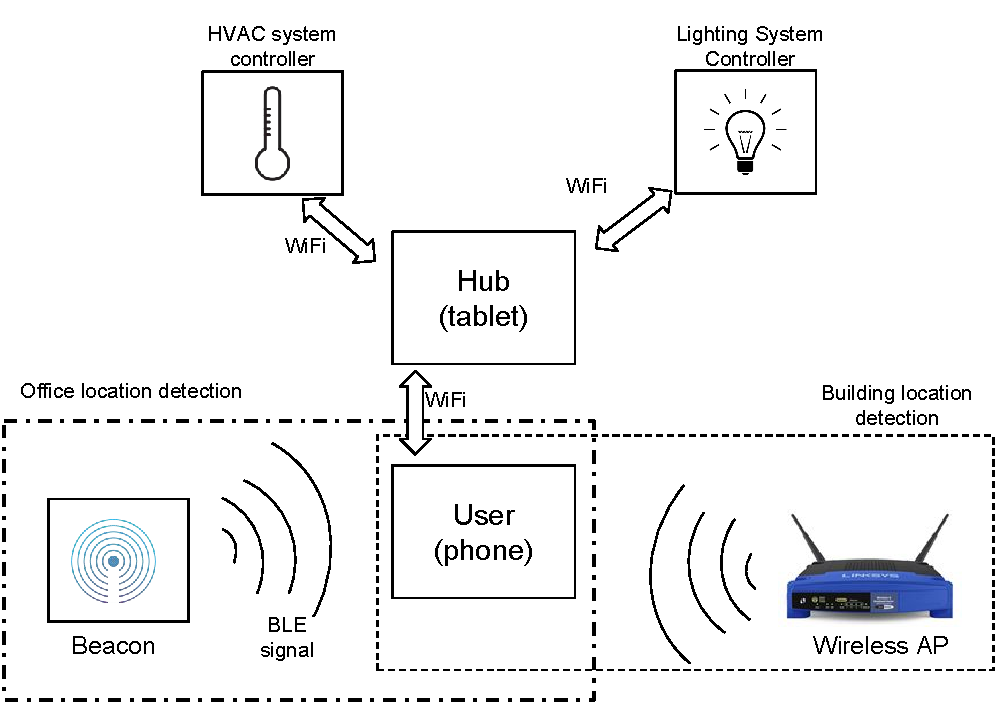
\includegraphics[width=0.4\textwidth]{Figures/harware_arch}
\caption{Overview architecture of the system}
\label{software1}
\end{figure}

\textbf{The Hub app} is responsible for controlling the \ac{HVAC} and lighting systems in the office, enforcing energy saving policies, improving occupant comfort and providing security monitoring when the user is away from the office.

The main visual features of the Hub application are: a simple \ac{GUI} to control the lights and heating/cooling system, an \ac{IFTTT} automation system that allows the user to create personalize trigger/actions rules. In the background it also provides motion detection and video recording for occasions when the user left the room but movement is detected.

\textbf{The User app} runs in the user's mobile device and offers remote control of the lighting, \ac{HVAC} and security systems provided by the Hub. Besides improving user comfort by allowing remote access to the Hub, the user app also helps the Hub with user detection, allowing the system to know when an authorized user is inside the building or room.

\subsection{Hardware Architecture}

To achieve building automation, our solution requires a tablet to act as a central control unit, a beacon device used for user detection inside the room and two other devices capable of interacting with the lighting and \ac{HVAC} systems. In Figure~\ref{hard_architecture_system} we describe the main hardware components of our system and the communication protocols used.

The tablet is where the Hub app is executed. It provides the sensors, the connectivity, the storage as well as a camera, microphone, speaker and a touch screen. 

The beacon is used for user detection, this will be explained later in Section~\ref{architecture4}.

To control the lighting and \ac{HVAC} systems we require devices capable of interacting with existing systems that offer a way to remotely control these existing systems. These devices can be for example microcontrollers. A microcontroller allows the digital world to interact with the real world through the use of actuators that convert electric signal into mechanical actions. The microcontroller is connected to the actuators (relay) and is able to switch on/off the lights as well as controlling the HVAC. This component is needed because typically, lighting and HVAC systems do not have any type of connectivity other than the electric wires. 

\begin{figure}[h]
\centering
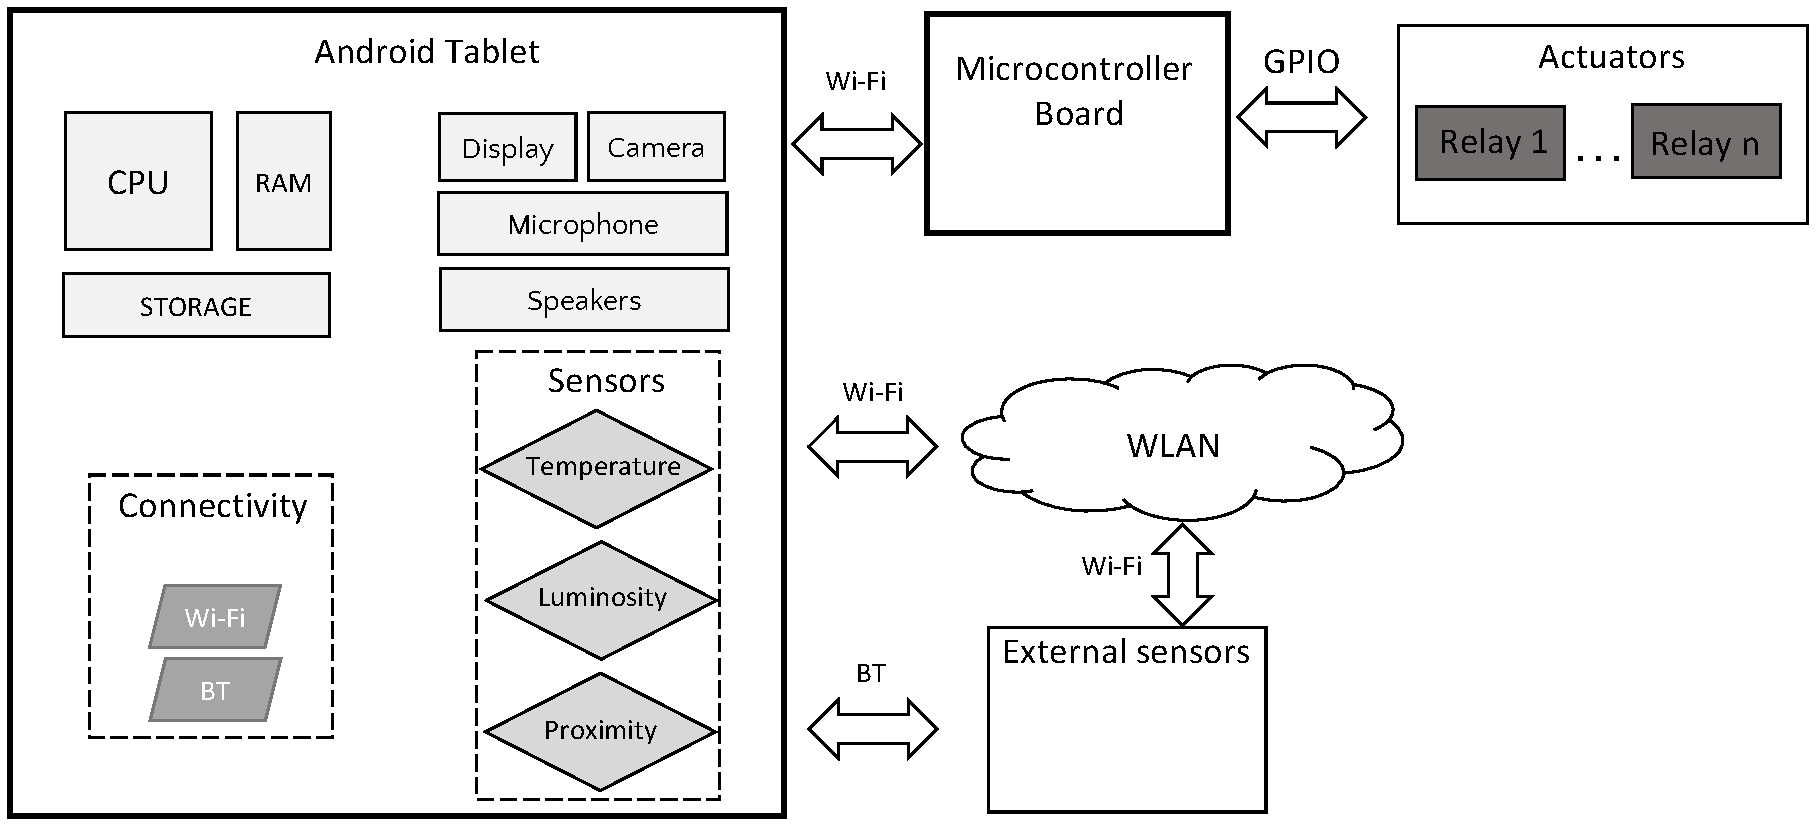
\includegraphics[width=0.5\textwidth]{Figures/arch_hardware}
\caption{Hardware architecture of the Hub}
\label{hard_architecture_system}
\end{figure}


\subsection{Software Architecture}\label{architecture4} 

In this section we present the software architecture for the mobile apps and explain some of the core functionalities of our solution.

To achieve \textbf{building automation} we propose a \ac{IFTTT} system. The user is able to create personalized chains of conditional statements, called "recipes", they are triggered based on events relevant to the office. With this system we could for example create a recipe that turns on the lights automatically when the user enters the room or shut them down when he leaves.

One of the goals of our solution is \textbf{user detection}, in order to accomplish this, we leverage two different types of location systems: \ac{WiFi} and \ac{BLE} beacon location. The location detection is handled by the user app. We use the building's \ac{WiFi} network to determine if the user is inside the building by comparing the \ac{MAC} address of available \ac{AP}s to a set of known addresses. The other location system we use is beacon location. There can be a beacon emitting \ac{BLE} signals and when this signal is detected, we know the user is near the beacon source (the office).

Regarding \textbf{office security}, we propose using the tablet's camera and analyzing the consecutive frames for changes. When no user is present in the room and a large enough number of pixels are different, we assume movement has occurred. We can then notify the user that someone is inside the room.


\subsubsection{Hub App Architecture}

We divided the Hub app into several managers, each responsible for several task. Figure~ \ref{software2}, represents the architecture of the Hub App.

\textbf{The \ac{UI}} must have a set of screens that offer:

\begin{itemize}
  \item Manual control of the lighting and HVAC systems.
  \item User registration.
  \item Creation of automation rules.
  \item Real-time ambient sensors readings.
  \item Security settings, enable/disable security monitoring and notification email.
  \item General settings, activate voice control, allow sound.
   
\end{itemize}

\textbf{Communication Layer}: The Hub app implements a web server offering an \ac{REST} \ac{API} that the user app can use to interact with. 

\textbf{The Event Manager} offers publish/subscribe service. It allows other managers to register their interest in certain events and when those happen they are notified. There can exist several different types of events: temperature reading, motion detected, user detection, etc.

The Event Manager is also responsible for the automation logic by enforcing the \ac{IFTTT} rules. The Automation Manager will check if the condition for the rule has been satisfied and trigger the action. Finally it also has a scheduler responsible for executing repetitive tasks at regular time intervals or at fixed moments.


\textbf{The User Manager} handles user registration, authentication and detection. It tracks the whereabouts of the user inside the building, in association with the User app so that, it is notified when the user enters the building or office.


\textbf{The Sensor Manager} allows access to the tablet's sensors as well as the external sensors. It abstracts external sensors into virtual sensors. It is responsible for a virtual motion detection sensor, by using the camera to detect changes that would indicate motion, as well as other data such as the opening and closing of the door.


\textbf{The Lighting Manager} is responsible for managing the lighting system. It communicates with the lightning controller (microcontroller) and synchronizes the lights state with the \ac{UI} and vice versa.

\textbf{The Temperature Manager} periodically reads the room temperature and is able to communicate with the \ac{HVAC} controller (microcontroller) to turn on/off the system when required.


\begin{figure}[h]
\centering
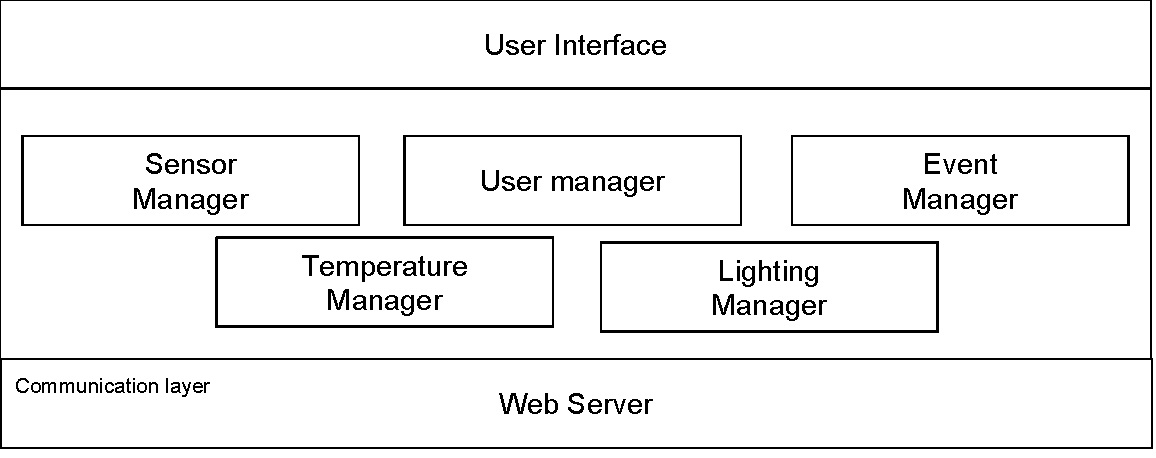
\includegraphics[width=0.4\textwidth]{Figures/software_hub}
\caption{Hub APP architecture }
\label{software2}
\end{figure}



\subsubsection{App Architecture}
The User App is simpler than the Hub App, the app is divided in \ac{UI} screens. There are no managers like the Hub architecture, the business logic is handled by each screen separately. 

The main screens are the home, lighting, temperature, security and registration screens.

Since the user app can control several Hub apps, we require a simple registration process to add the user to the Hub. We propose showing a QR-Code in the Hub registration screen, this code possesses the \ac{IP} address for the Hub and a temporary token used for registration. The user app can use the phone camera to scan the QR-Code and automatically register the user in the Hub. Then a virtual representation of the Hub is shown in the home screen.

For user detection to work when the app is not being used, we use a background service to monitor the \ac{WiFi} and beacons nearby the phone. The interval between scans are one every five seconds for \ac{BLE} scans and one minute for WiFi, these values are adequate times between scans to be conservative regarding the user's mobile device battery.



\section{Implementation}

This section addresses the main decisions adopted regarding the implementation of BASA.
Thus, the following sections cover the hardware and software choices made in the development process of BASA.

\subsection{Hardware Architecture}\label{hardware_arch_imp}

In Figure~\ref{imp:architecture_system} is shown the required hardware components of our system. We require tablet to run the HUB app, an optional user phone with a User app installed, a device to control the HVAC system (two supported Arduino HVAC or PerOMAS\cite{peromas}), a Edup smart light switch to control the lights. We also need a \ac{BLE} beacon for user detection inside a room and require the building's \ac{WiFi} network for user detection inside the building.
To allow communication between different components in the system we use the building's \ac{WiFi} network for local communication and use Firebase servers to allow external access from outside the building's network.


\begin{figure}[h]
\centering
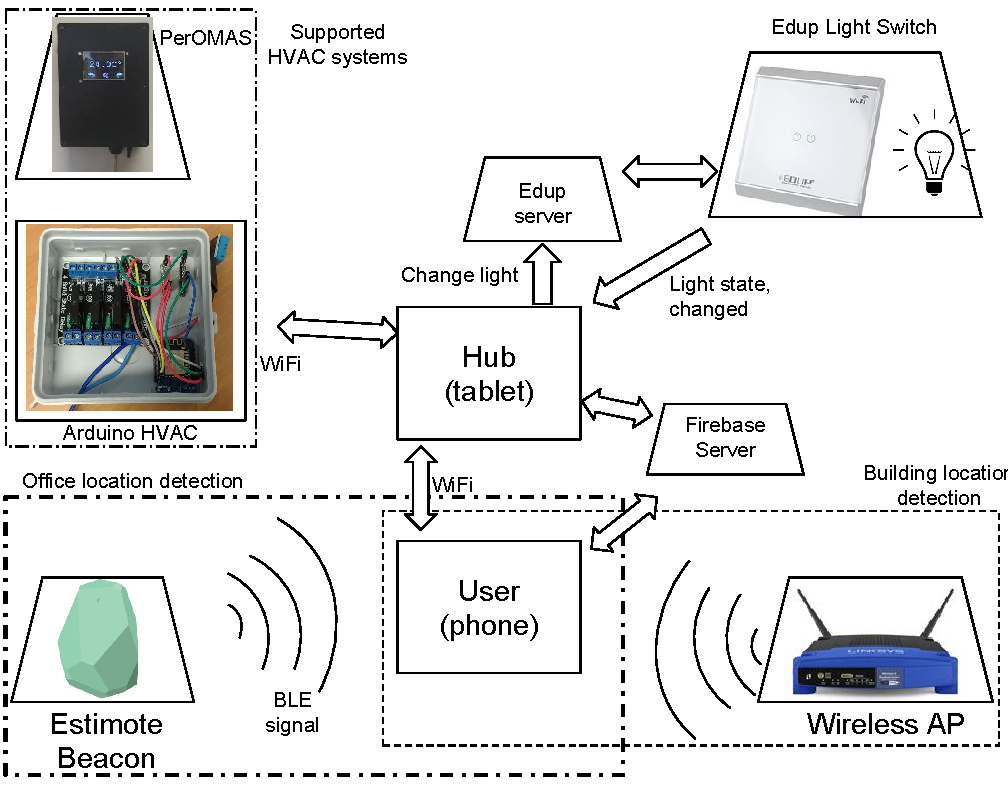
\includegraphics[width=0.4\textwidth]{Figures/harware_arch_imp}
\caption{Hardware implementation architecture}
\label{imp:architecture_system}
\end{figure}

\textbf{Tablet}: We decided to use the Nexus 7 (2013) Android tablet as the base of our solution. We compared IOS, Android and Windows devices and concluded that an Android tablet fitted our needs.

\textbf{HVAC control}: In order for our \ac{BAS} solution to control an \ac{HVAC} system, we need to either communicate with a building central controlling unit or physically control the system like a thermostat does. Since most buildings don't have a central control point running some kind of server where you can control it using the Internet, we went with the thermostat route.

We compared several thermostat alternatives with WiFi capabilities and concluded there was none that fitted the requirement of low cost. We decided to make a Arduino based device with built in \ac{WiFi}, a relay to drive the electric wires and a temperature and humidity sensor. 

Besides the mentioned Arduino based solution some offices in our University have installed the PerOMAS automation system that allows remote control of the installed HVAC system. Due to time constraints the Arduino base solution was not installed and we used PerOMAS for HVAC control instead.





\textbf{Lighting control}:
Besides controlling the room \ac{HVAC}, we require control over the lighting system. After some research we had three options: using wireless controllable light bulbs, using some kind of Arduino/relay solution (like the thermostat) or using a wireless controllable light switch.

Our lighting solution should be affordable, have a physical light switch and an API to control it. The smart lights were not supported by our office (fluorescent tube lamp) for these reasons we excluded them, also the Arduino based solution implied assembling the components and that should be kept to a minimum to make BAS more easily deployable.

The lighting option chosen was the Edup Smart Light Switch. It provides a physical light switch, supports the existing infrastructure in the buildings (as long as there is a phase and neutral wire in the wall socket) and is not too expensive.


Originally we proposed to have, the lighting system integrated with the Arduino/\ac{HVAC} using relay actuators. In the end we decided go with the Edup light switch after searching for lighting products we could control, it is a better solution because of the touch control, the ability to continue to use the lights in case of system failure (no Internet or control mobile application crash) and no need for assembly as described previously.

Unfortunately the wall socket where the light switch was going to be installed was missing the neutral wire and the wait time for electricians to wire the neutral wire to the wall socket would take too long. The alternative found was to use the light switch to control a lamp, as shown in Figure~\ref{imp_light_switch_light}.


\begin{figure}[htbp]
\centering
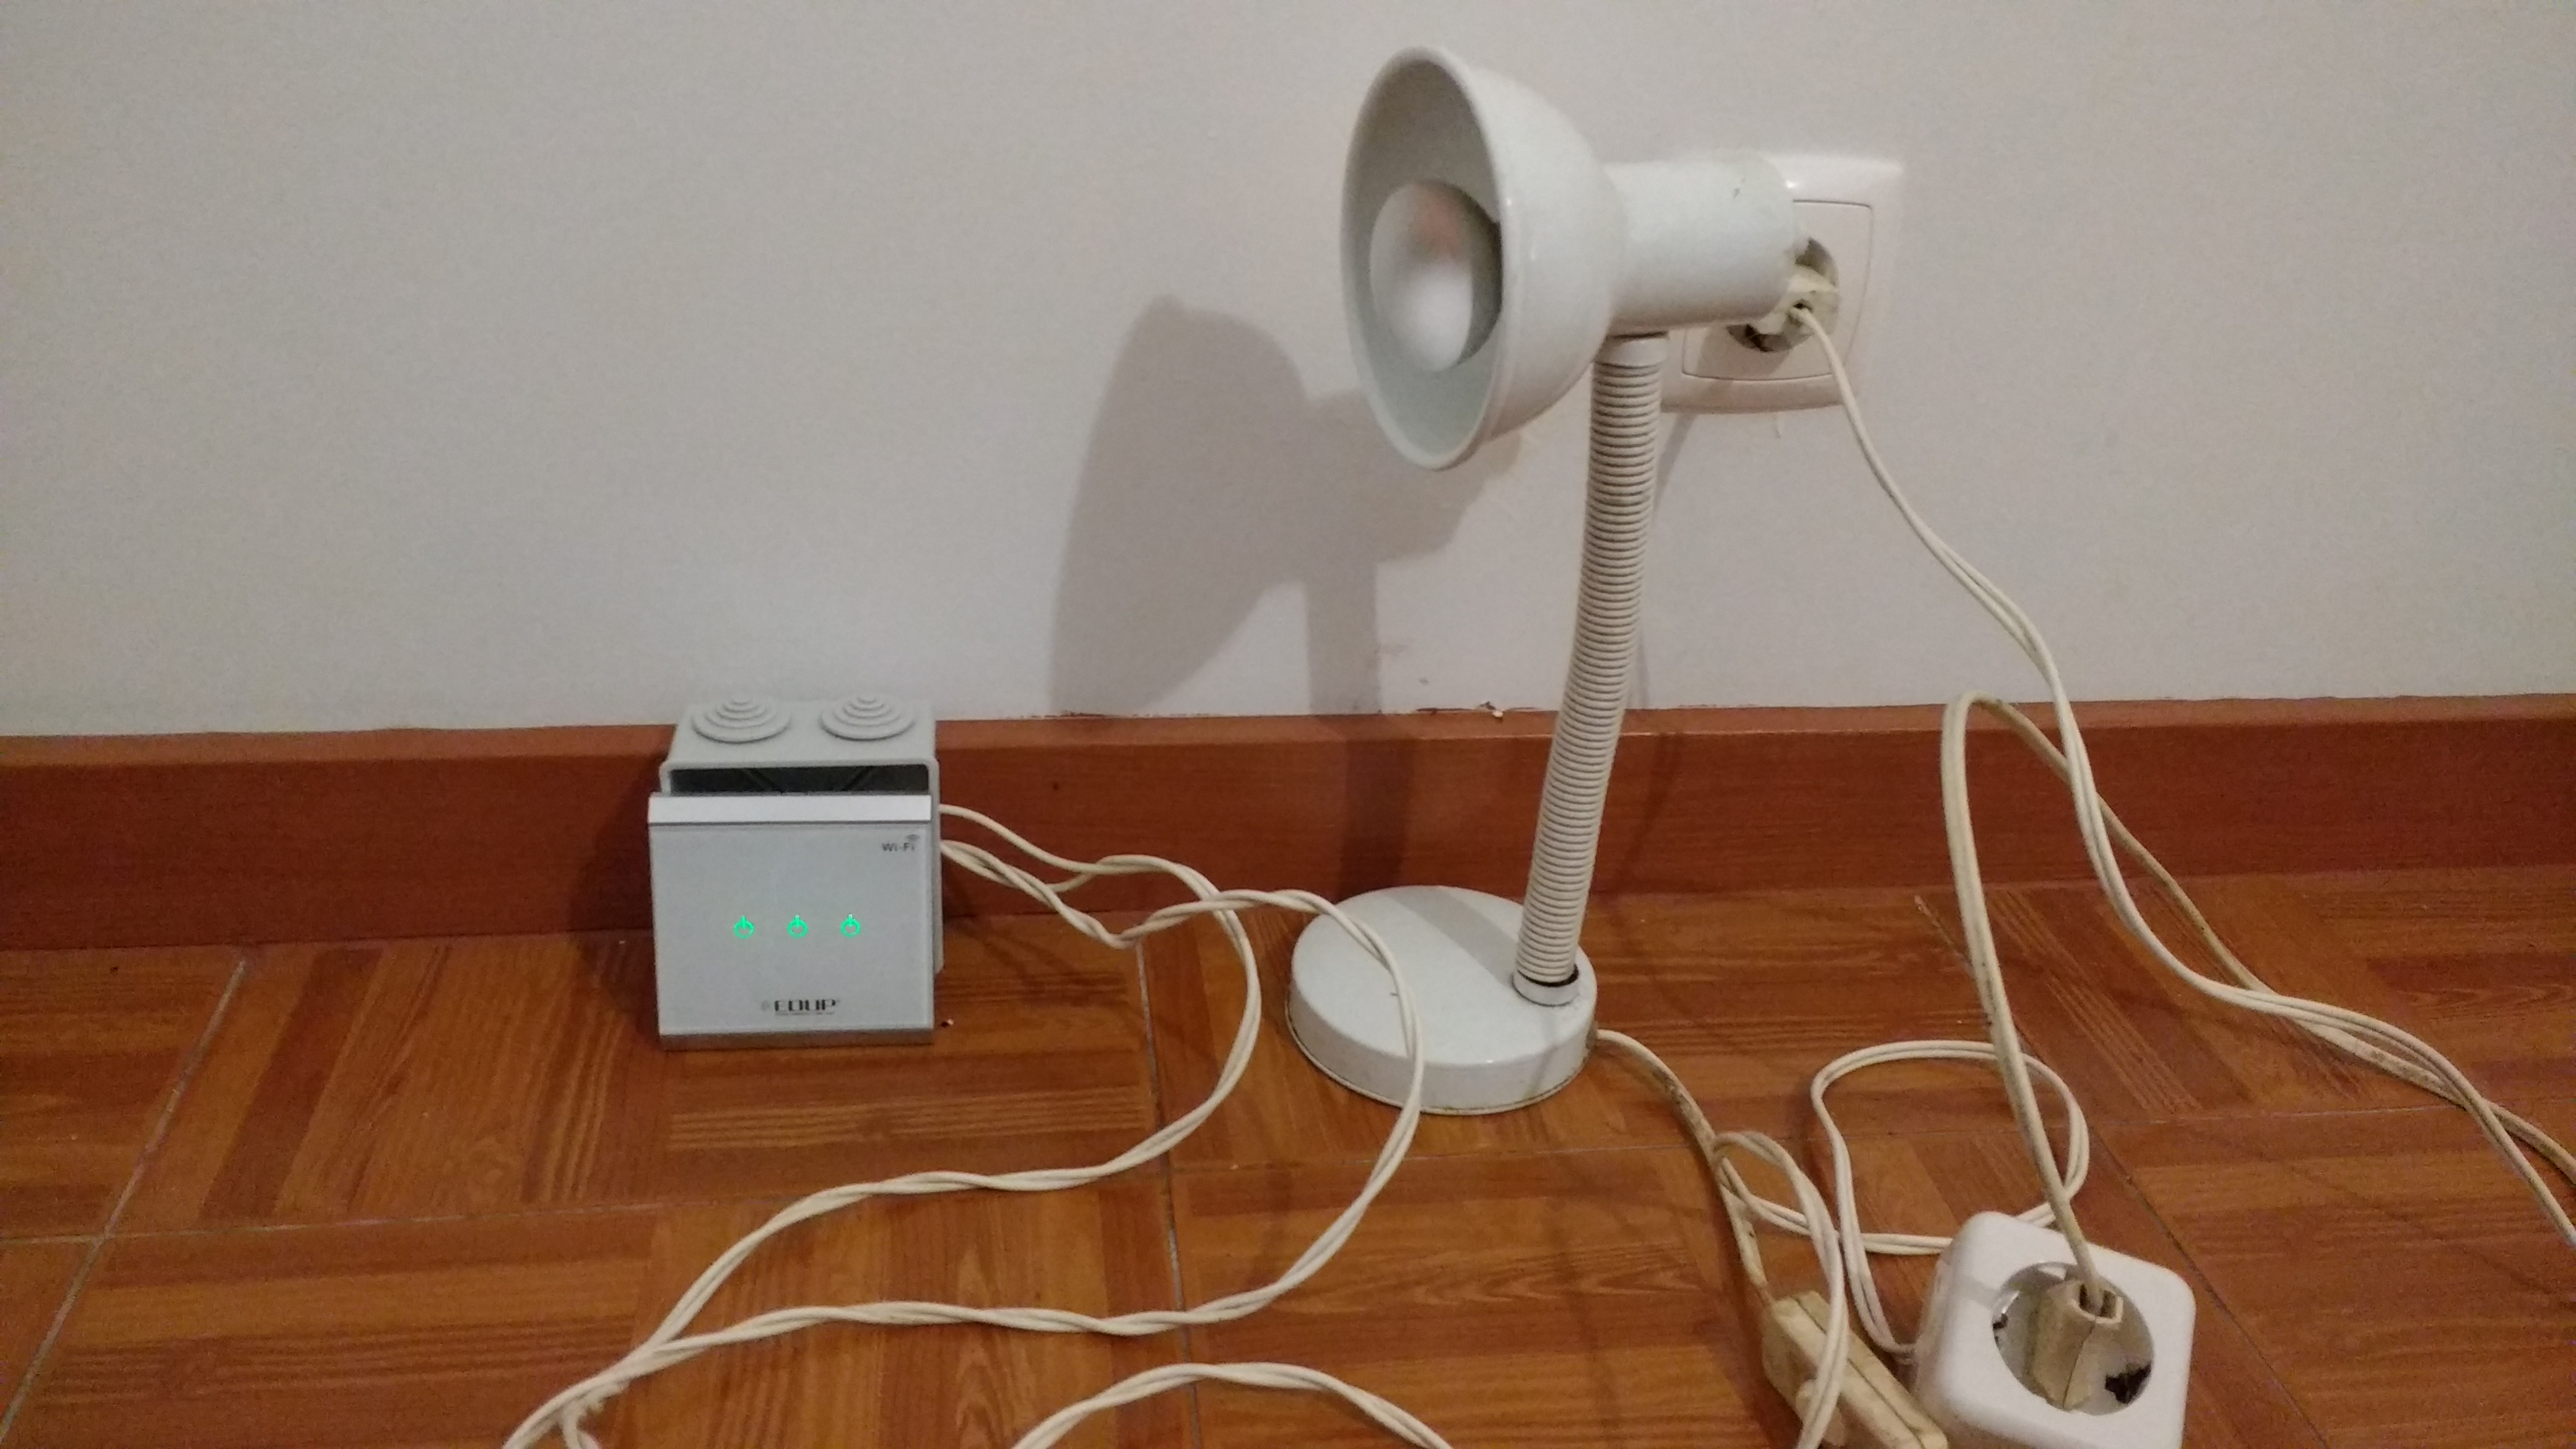
\includegraphics[width=0.25\textwidth]{Figures/imp_light_switch_light}
\caption{Edup Light Switch connected to a lamp to simulate room lights}
\label{imp_light_switch_light}
\end{figure}


\textbf{Bluetooth Beacon}: We require a way to determine if a user is near a certain point in the building such as the office.

From the alternatives seen in Section~\ref{rel}, we  determined that \ac{BLE} beacons are an option to achieve room level location in a building.

There are many kinds of devices capable of emitting \ac{BLE} packets: android devices( available in version 5.0), some microcontrollers and commercial beacon products.

We decided to use an Estimote beacon. One reason it was chosen was because we had access to one and did not need to buy it. This beacon also has the advantage of providing temperature readings if needed. Since it is portable we can position it anywhere in the room, enabling better coverage.


\subsection{Software Architecture}

Our solution is divided into two separate Android applications, the Hub and the User apps. Both apps work side by side in order to achieve the following functions: user detection, control over \ac{HVAC} and lighting systems, task automation and finally video monitoring \& security. These functions are the building blocks which enables our solutions to achieve building automation, increase user comfort and security monitoring.


\subsubsection{User Detection}\label{user_detection_imp}

One energy wasting problem is having lighting and \ac{HVAC} systems turned on when no one is present.

In order for our system to take informed actions to cut wasted energy consumption, we need to know the location of users inside the building.


The location detection is handled solely by the User app. After it confirms the user is inside the building or office it communicates with the Hub. The Hub on the other hand has a timeout system. When a user fails to communicate for a certain amount of time, we presumed he is outside the office or building.

\mbox{}\\
\textbf{In the building}

The building location detection consists in scanning the available \ac{WiFi} networks and checking if the \ac{MAC} address of the \ac{AP} matches a list of pre-scanned \ac{AP}s. Scanning for \ac{AP}s is battery draining and should be kept to a minimum. We decided to start scanning only when the phone connectivity changed. For example when a user enters a building his phone connects to a known \ac{WiFi} network. We use this event to start scanning if the user is inside the target building. If after the first five scans (5 minutes) no matching \ac{MAC} address is found, the scanning is disabled until a new connectivity change happens. 

\mbox{}\\
\textbf{In the office}

There is an Estimote beacon in the office broadcasting a \ac{BLE} signal. The User app is scanning for these signals and when one is found, it checks if the namespace in the beacon package matches the known office namespace. After a correct match is found the User app informs the Hub the user is near the office.

While \ac{BLE} is a lower-energy system than traditional \ac{BT}, scanning is still a fairly power-intensive operation. To limit the battery drain, we only start scanning when the user is in the building and stop after he leaves.

\subsubsection{Lighting control}\label{light_imp}


The lights in the room are controlled by the Edup Light Switch. The switch must be connected to a WiFi network and automatically establishes a connection to Edup server to enable remote control over the switch. There is no official \ac{API} available to control the switches. In order to understand how the light switch worked, we used Wireshark to sniff the traffic created by the Edup app and tried to replicate the messages.

To control the light switch we must open a \ac{TCP} socket send a packet with the data shown in Figure~\ref{edup_imp} to Edup server.

Since there is a physical light switch interface we must update our application status if a button is pressed outside our app.
The Edup Light Switch sends a \ac{UDP} multicast message when the lights are changed. We implemented an \ac{UDP} server to listen for those messages. 



\begin{figure}[h]
\centering
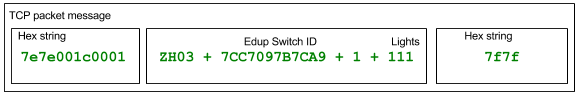
\includegraphics[width=0.4\textwidth]{Figures/Edup_imp}
\caption{Edup packet to set the light state.}
\label{edup_imp}
\end{figure}




\subsubsection{HVAC control}

Our HVAC solution uses an Arduino with a webserver to control a relay in order to interface with the existing HVAC system.

The Arduino we implemented to control the HVAC system was written using C++ programming language. It has four jobs: run a webserver to allow remote control, implement \ac{SSDP} to enable discovery, read temperature/humidity values from a DHT11 sensor and control a four relay module to control the HVAC system.

After the device is first powered up it becomes an \ac{AP}. The user must connect to this new network and use the browser to choose the \ac{WiFi} network he want the Arduino to connect.

There is a discovery mechanism to add the Arduino IP address automatically to the Hub app. Our Arduino based HVAC is programmed to be discoverable using the \ac{SSDP} protocol using a search target equal to "schemas-basa-pt:service:climate:1".

BASA can also control the PerOMAS system installed in some offices in our campus, we communicate with PerOMAS using it's web-server.

\subsubsection{Automation}

One of the goals of BASA is enabling the automation of lighting and \ac{HVAC} systems. A simple example of an automation task is turning off the lights when no occupant is inside the office.
With our system we aimed to give the user high control and flexibility over the automation process. We allow the user to create chains of simple conditional statements, called "recipes", which are triggered based on events relative to the office.

The recipes contain a list of triggers and actions. A recipe can have one or multiple triggers, when there are multiple triggers we use the logical AND operator, all the triggers must be true in order for the recipe to be triggered.

There are seven triggers available:

\begin{itemize}
  \item \textbf{Temperature:} This trigger allows the user to trigger an action when the office temperature is below or above a value specified.
  \item \textbf{Motion:} The motion sensor is triggered when something changes in the field of view of the Hub or no movement detected in X seconds.
  \item \textbf{Speech:} Say the keyword "my assistant" and after the beep you say the phrase specified in the trigger.  
  \item \textbf{Time:} The timer trigger allows the user to run certain actions at a specific time(Scheduler).  
  \item \textbf{User location:} Allows actions to be triggered based on the user location
  \item \textbf{Light sensor:} The light sensor triggers an action if the light level is below or above the value specified.
  \item \textbf{Light state:} This trigger allows the user to trigger an action when the lights are in a specific state.
  
\end{itemize}

The actions available are:

\begin{itemize}
  \item \textbf{Light:} Sets the state of the lights.
  \item \textbf{Temperature:} Changes the target temperature and turns on the HVAC if needed.
  \item \textbf{Speech:} This action uses the speakers to say the text specified (text to speech).
\end{itemize}

In order to show the flexibility of our solution we created the following example recipes:
\begin{itemize}
  \item If a user is in the office and the temperature is above 25ºC then we turn on the cooling.
  \item If no user is inside the office then turn off all the lights and the HVAC.
  \item If the user says "turn on lights" then turn on all the lights.
  \item if the user location status is "user arrives at office", then say "Welcome back".
 
\end{itemize}








\subsubsection{Communication}

BASA has several devices that need to communicate with each other as well as external services. To allow communication we implemented the following services:


\textbf{Rest server (Hub app)}: We implemented the server using java and the SPARK 1.1.2 framework \footnote{http://sparkjava.com/} running at port 5002.

The server exposes a Rest API that allows the User app to communicate with the Hub.

\textbf{Rest client (Hub and User app) }: The Rest client  uses the Retrofit Android\footnote{https://square.github.io/retrofit/}  library to allow our apps to initiate communication with a server. It is used by the User app to interact with the Hub app server and used by the Hub to communicate with the Arduino, PerOMAS and Weather forecast API.


\textbf{Firebase (Hub and User app)}

Originally the plan was to only use the web server, but in our building we can't run web servers in the WiFi network. When we tried to contact the Hub it did not receive any request. Then we changed to a private wireless network it all worked normally.

The solution we found for connecting  to the Hub when the User app is outside the \ac{WLAN} was Google Firebase. It is a platform that offers multiple services. We use two services, the real-time database and the storage.
We use their real-time database to synchronize application data across clients and store it on Firebase cloud. The application data we store are the temperature, the temperature the thermostat is set to, the light state, the beacon namespaces and MAC addresses for user location and finally data related with live camera view of the office and recorded videos storage location URLs. The storage service is used to upload the recorded videos and live preview images, captured by the security system.

Firebase solves us two problems, one is users can access our solution from home and access the live camera, Firebase is used as a middleman to communicate. The second problem it fixed was user detection, since our building is big, the private network where the tablet is connected can't be access in most of the building. A user entering the building could not communicate with our Hub and notify of its presence since they were in different networks. We use Firebase to add our location messages that are then received by the Hub to achieve and building level user detection.

\subsubsection{Security - Motion detection, video recording, Live view}\label{imp:security_motion}

With our office being like an extension of our home, we felt the need to have some sort of video surveillance system. We created a system capable of detecting if a object is moving inside the office, identify if a user is inside the office and if not, send a notification to the user and record a small video.

\textbf{Motion detection}: The motion detection works by comparing two camera frames. If a percentage of pixels are different we assume motion has happened. Both the percentage of different pixels and the detection period are configurable using the \ac{UI}.

In order for a camera frame pixel to be considered different the RGB value of the pixel must vary more than 50 in a scale between 0 and 255. The percentage of different pixels for a positive detection is user defined, the default is 0.5\%.


\textbf{Video recording}: When motion is detected and no user is inside the office we record 30 seconds videos. We do not record constantly, just after motion is detected. These videos are uploaded and stored to Firebase servers, where the user can later watch them using the user app.

\textbf{Live Camera}

We can watch in real time pictures from the office camera. When the user is using the User app live camera functionality, the Hub saves a camera frame every second to the Firebase server. We have seen a minimum delay of 4 seconds between the live pictures and the time they were taken.



\subsubsection{Hub app}

The Hub app suffered a few changes from the initial architecture with the addition of more functionalities.

We added two more managers to the Hub app: 
\textbf{The Speech Recognition Manager} was inspired by Amazon Echo product and offers our users voice recognition. This new feature is currently used with our automation solution to allow the user to trigger recipes using voice commands. 

This manager uses the CMU Sphinx\footnote{http://cmusphinx.sourceforge.net/wiki/} offline keyword speech recognizer. When it detects the keyword, it shuts down and we launch Google online speech recognition. We use this other speech recognition because it offers better results, the reason the manager uses two different speech recognizers is because using only Google recognizer has higher bandwidth cost since we would be constantly sending audio. 

\textbf{The Video Manager} does two jobs, it records 30 seconds videos when no user is present in the office and motion is detected. The other job is offering a live preview of the office, an user can use the user app to watch in real time the office.



\textbf{User interface}: The final \ac{UI} of the Hub app is composed of three main screens: a lighting screen, a temperature screen and general menu that contains several advanced features.

The \textbf{lighting screen}, allows the user to control the lighting environment in the room.

The \textbf{temperature screen}, shown in Figure~\ref{screen_temperature} gives visual information about the current weather outside. There is also a virtual thermostat where the user can select the temperature he desires. 


\begin{figure}[h]
\centering
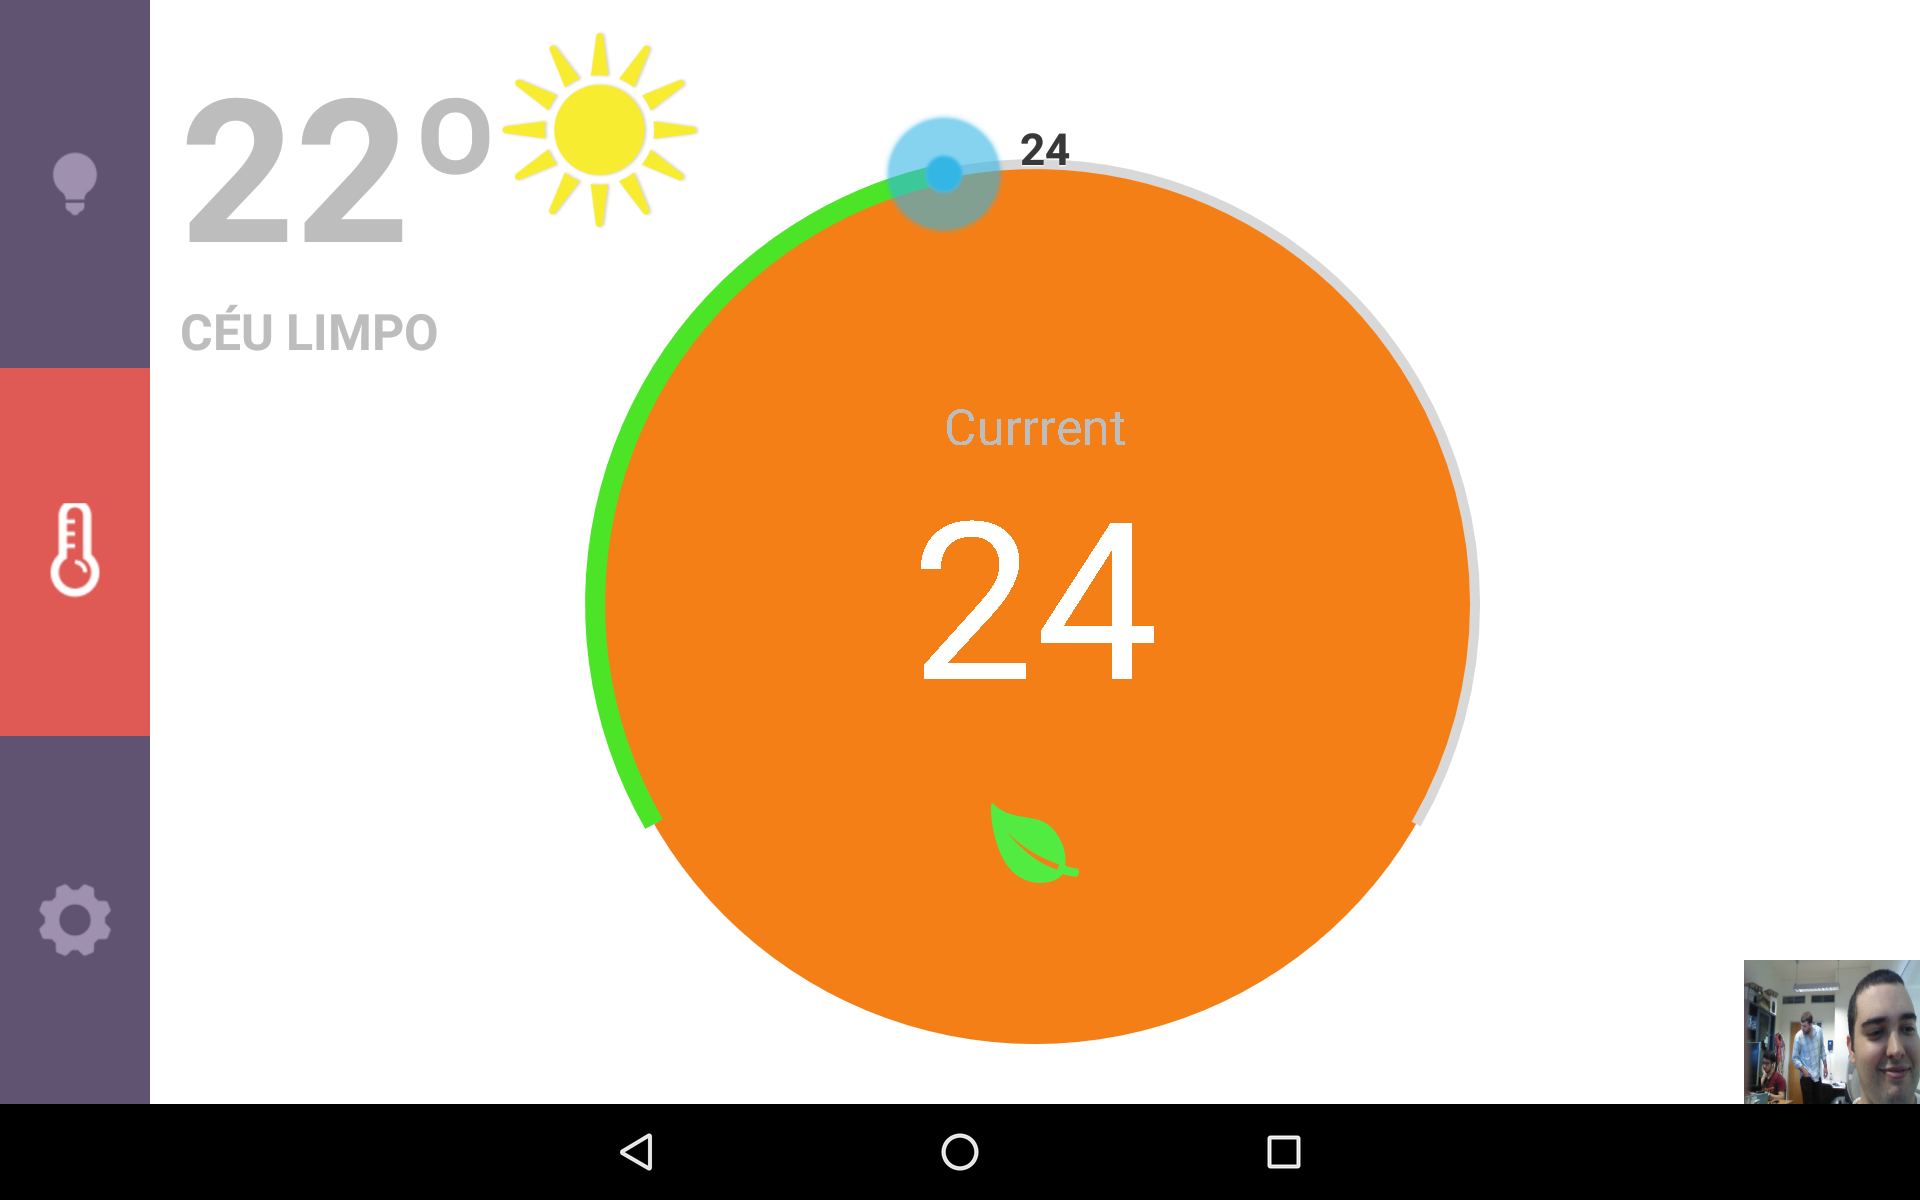
\includegraphics[width=0.3\textwidth]{Figures/screen_temperature}
\caption{Temperature fragment.}
\label{screen_temperature}
\end{figure}


There is a \textbf{general menu} that contains the other screens that enable additional features. This menu contains:
\begin{itemize}
  \item \textbf{User registration:} Allows a person to setup an account in Hub.
  \item \textbf{Recipe management:} Contains a list of the current recipes in the Hub and allows the user to create, edit, disable/enable and delete them.
  
  \item \textbf{Event history} Shows a list events ordered chronologically.
  
  \item \textbf{Statistics screen} Shows temperature, lighting status, luminosity and occupation graphics.   
  
  \item \textbf{Settings screen} Allows the user to configure the Hub app.
\end{itemize}



The \textbf{user registration screen} allows the user to register using the user app or an email address.
If the user uses the Android user app, a visual registration token is shown in the form of a QR-Code. The QR-Code contains a temporary id and the IP address of the Hub server. This temporary id is later needed when the user registers and exists to ensure only people inside the office can register and not just anyone that knows the IP address. If the user chooses to register with just the email we use Maingun\footnote{http://www.mailgun.com/} API to send a email to the provided email address with a identification QR-Code for user login.

In the \textbf{recipe screen}, the user can create new recipes, first the trigger/s is selected, only then can the action/s be picked. Figure \ref{screen_completed_recipe} shows one of the screens to create a recipe. 

\begin{figure}[h]
\centering
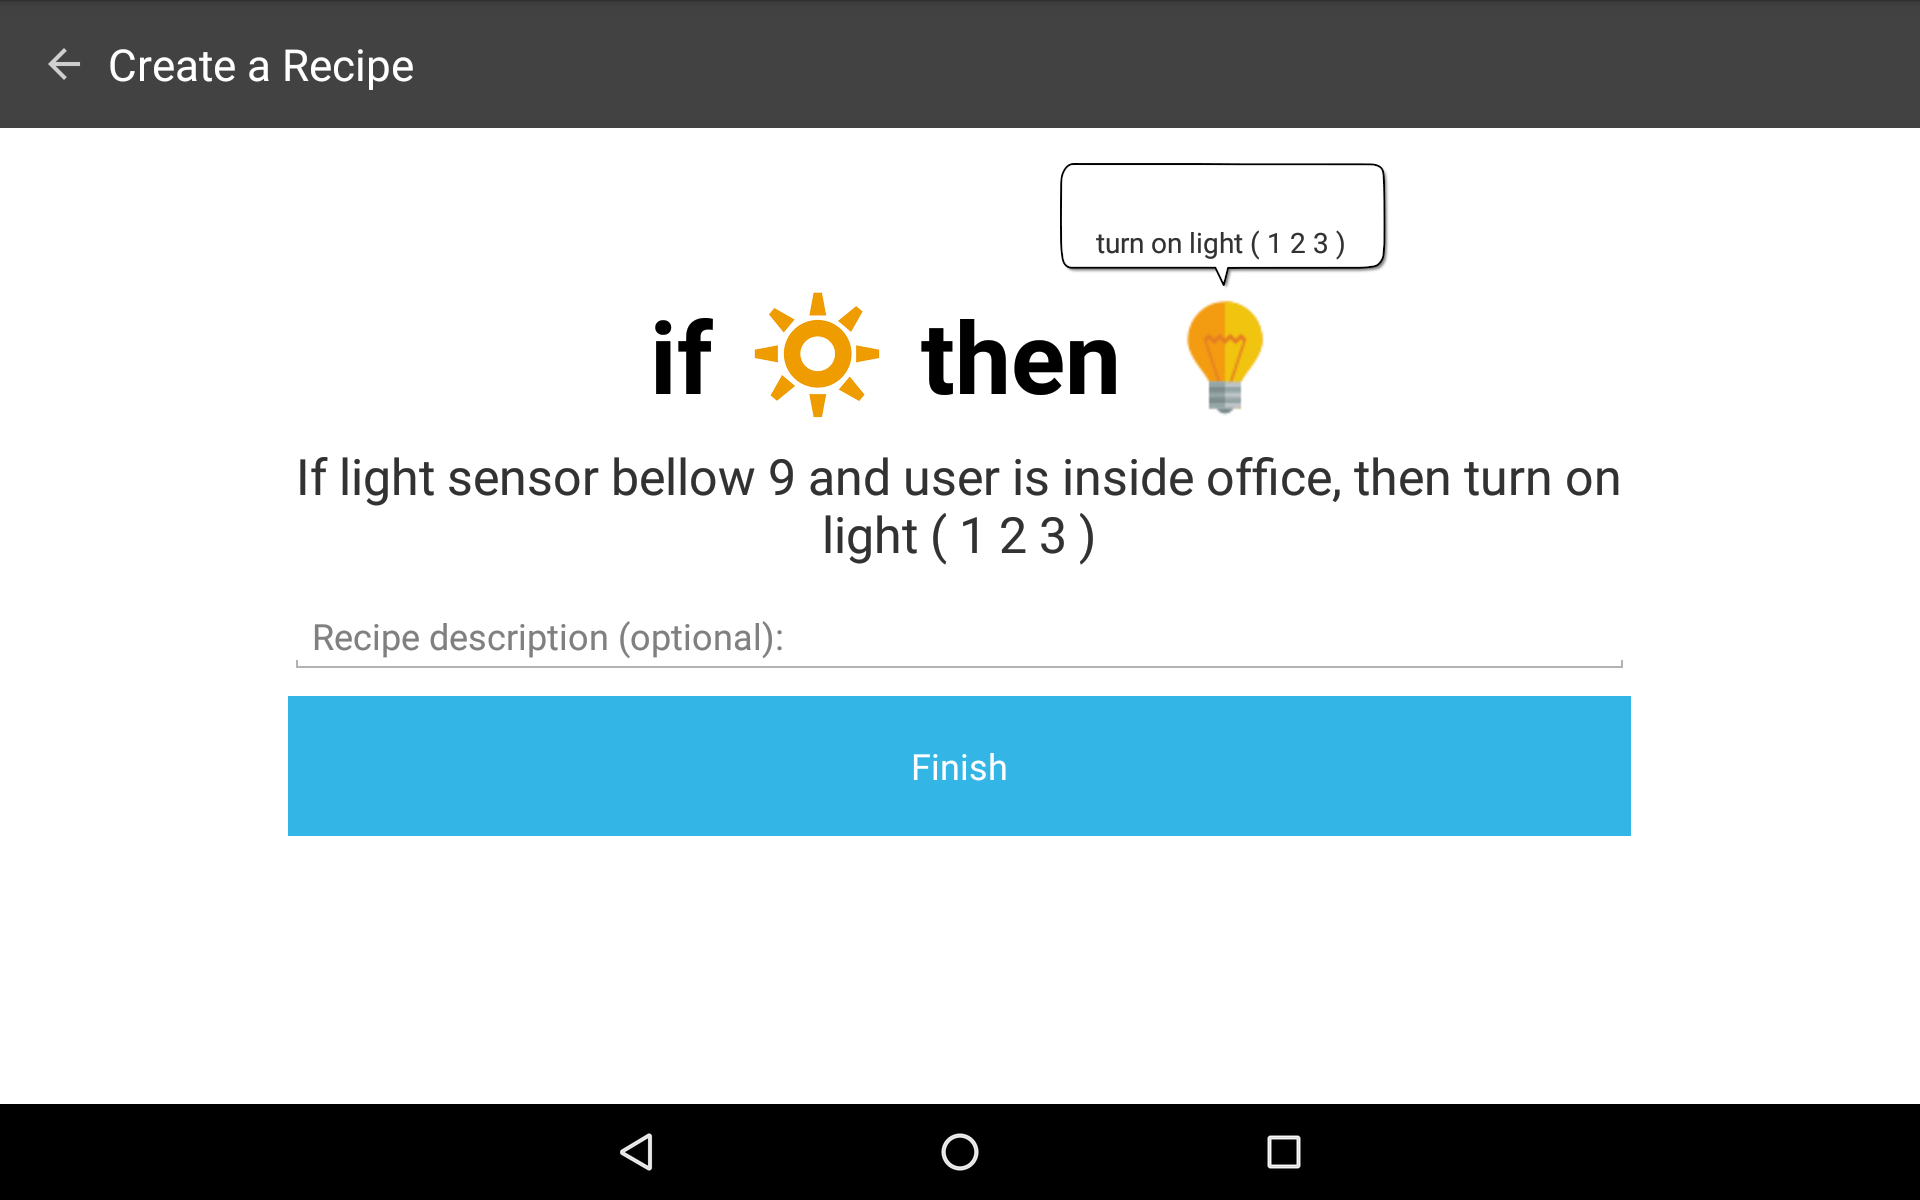
\includegraphics[width=0.3\textwidth]{Figures/screen_completed_recipe}
\caption{Final recipe creation fragment.}
\label{screen_completed_recipe}
\end{figure}

The \textbf{settings screen} allows the user to configure many different parameters in the app, this screen also allows the user to:
\begin{itemize}
 
  \item Specify an area in the camera frame where motion is ignored.
  
  \item Scan for Arduino/HVAC, shows the list of available Arduino based HVAC in the network.
  
  \item Enable Kiosk mode, this mode disables the home and power button of the Android device. It prevents a user from closing the app. 
    
  
\end{itemize}







\subsubsection{User app}


The User app allows user detection, remote control over the office, access to live image preview of the office, notifications when movement is detected, and video history of recorded videos.

The User app allows the user to create zones, in a zone the user can add and control Hub devices. To add a device the user uses a screen with a camera and scans the Hub app Qr-Code available in the Hub's registration screen.
After the Hub device is added three icons representing three services appear in the zone screen: control lighting, \ac{HVAC} and security systems. This is shown in Figure~\ref{imp_user_app}.

The lighting and \ac{HVAC} screens are straightforward, they allow the user to remotely control a Hub's lighting and \ac{HVAC} systems. The security screen enables live camera visualization of the Hub's camera and access to a list of recorded videos. When motion is detected by the Hub all registered users are notified via Android notification. 


\begin{figure}[h]
\centering
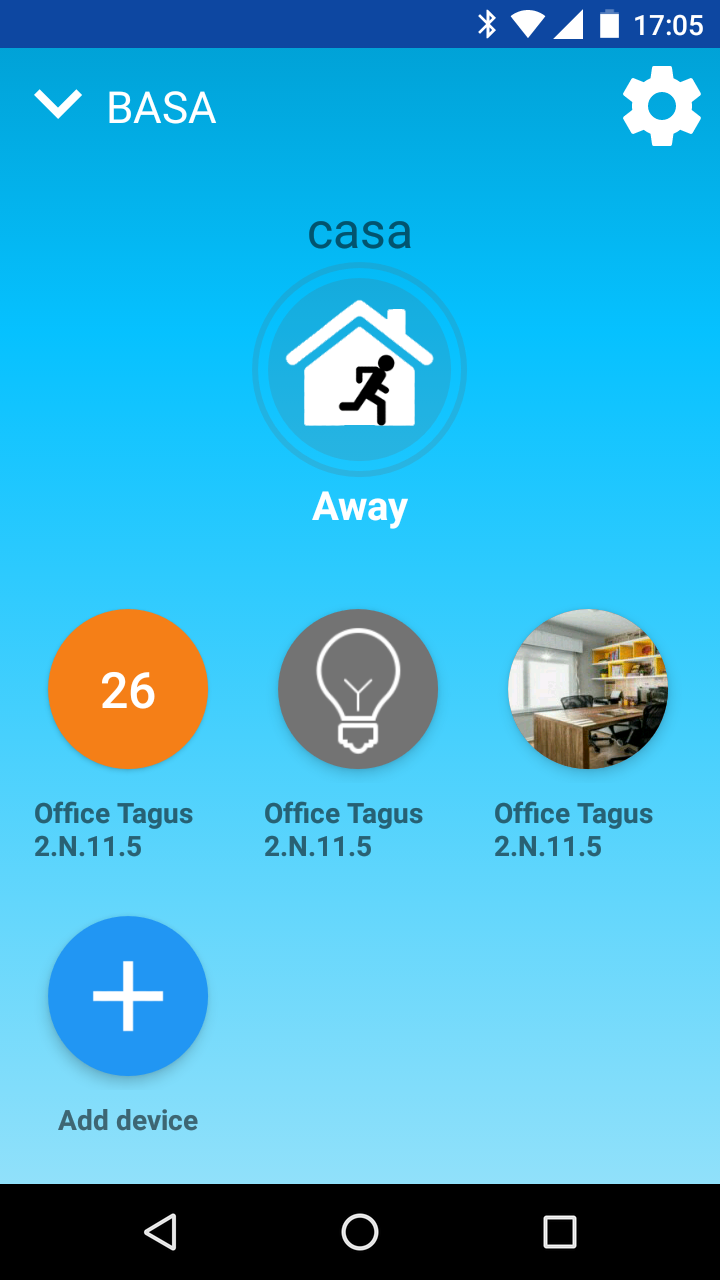
\includegraphics[width=0.15\textwidth]{Figures/imp_home_user_app}
\caption{HomeFragment screen with the added Hub.}
\label{imp_user_app}
\end{figure}


\section{Evaluation}

In order to evaluate the developed solution, we deployed the BASA system in one office. Our goal was to validate the basic operation  of the system and it's ability to provide energy savings through user detection and automation. Provide its users with their desired temperature settings. Test the motion detection system developed. Finally evaluate the \ac{UI} of the automation solution developed.

All the tests were made using an Android Nexus 7 2013 tablet, a motorola Moto G3 Android phone, the Arduino based HVAC with a DHT11 temperature sensor and a Estimote BLE beacon.

\textbf{User detection - Room}: We measured the time it took the User app to detect the BLE beacon inside the office, the user was initially outside the office and entered the room starting the timer. The cumulative distribution function for the test is shown in Figure~\ref{eval:room2}.

We observed that in most cases our system detected the user presence very quickly within few seconds but in other occasions it seemed to take up to 30 seconds. We noticed once it detected the Estimote beacon the first time it found it correctly the following times but, seems to take some time for the initial discovery. We consider that the time to detect the user presence is adequate for turning on the \ac{HVAC} system in the user presence but not perfect for turning on the lights when the user enters the room.

For cases when the user wants the lights to be on when he enters the room and if the detection time is considered insufficient, a automation recipe can be created for turning on the light when movement is detected and the user is inside the building. Nevertheless, we consider the room detection time adequate for rooms with ambient light from a window but not for dark rooms.


\begin{figure}[]
\centering
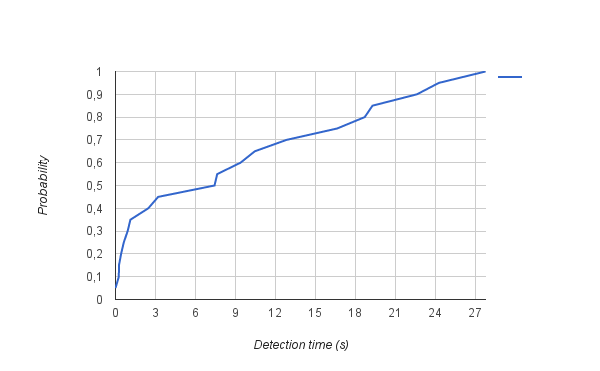
\includegraphics[width=0.5\textwidth]{Figures/room_detection_cumulative2}
\caption{Cumulative distribution function of the time it takes to detect a user when user enters room}
\label{eval:room2}
\end{figure}


\textbf{User detection - Building}: Several measurements were taken to determine the response time the application takes to identify the user is inside the building. The cumulative distribution function from the measurements is shown in Figure~\ref{eval:building1}.

Building level user detection does not need very quick response times, unlike room detection, as building location will be mostly used to preheat the room before the user arrives. The response time observed shows an acceptable response time.


\begin{figure}[]
\centering
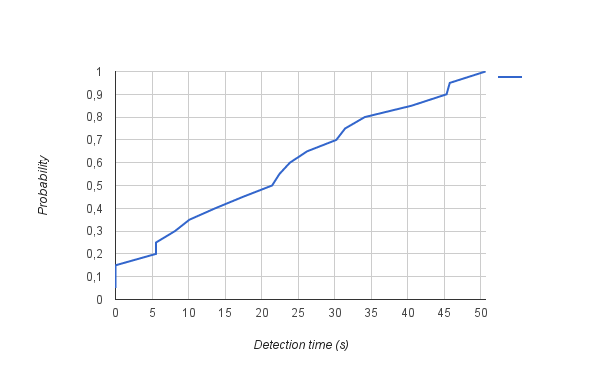
\includegraphics[width=0.5\textwidth]{Figures/building_detection_cumulative}
\caption{Cumulative distribution function of the time it takes to detect a user  after he enters the building}
\label{eval:building1}
\end{figure}



\textbf{Motion detection}: To test motion detection, we conducted tests with three different people with different heights. Each person entered the room at different speeds, the obtained results are shown in Table~\ref{eval:motion}.

Our system was able to correctly identify a person walking inside the room every time, Figure~\ref{eval:motion_fig} shows an example of the different pixels in the camera frames identified by our algorithm. Regarding false positives, from object motion they don't seem to be a big problem since our system allows the creation of a no-monitoring-area in the camera frame to use in cases of rooms with window view.

The motion test was performed during day hours, in these conditions the camera is able to capture good frames. We did not perform test during the night time  but it's likely our system will have problems detecting movement in completely dark rooms. To fix this problem we can install sensors to detect if the office door is open. If the door is opened and there is not enough light our system could turn on the lights momentarily to enable motion detection.


\begin{table}[h]
\centering
\begin{tabular}{|l|l|l|l|}
\hline
 & \begin{tabular}[c]{@{}l@{}}Person 1\\ detection\end{tabular} & \begin{tabular}[c]{@{}l@{}}Person 2\\ detection\end{tabular} & \begin{tabular}[c]{@{}l@{}}Person 3\\ detection\end{tabular} \\ \hline
Slow walk & 20/20 & 20/20 & 20/20 \\ \hline
Normal walk & 20/20 & 20/20 & 20/20 \\ \hline
Run & 20/20 & 20/20 & 20/20 \\ \hline
\end{tabular}
\caption{Motion detection tests for three people with different heights, 20 measurements each.}
\label{eval:motion}
\end{table}


\begin{figure}[h]
\centering
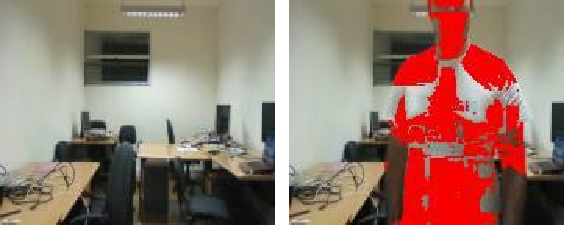
\includegraphics[width=0.4\textwidth]{Figures/eval_motion}
\caption{Motion detection - Frame before and after, motion detected }
\label{eval:motion_fig}
\end{figure}

\textbf{Temperature and Luminosity}: In order to test the functionality of the luminosity and temperature sensors in the system, these were used to collect ambient data.

To test the luminosity sensor behavior, we turned on the lights in the room and allowed the Hub to record the values for a while, then we turned off the lights and waited for a few minutes then repeated the same steps one more time. In Figure~\ref{eval:lights} we can observe two different gaps where the lights were off. As expected the Android luminosity sensor operates as intended and provides the system with correct data. 

To test the external temperature sensor, the HVAC system was turned on and the temperature was recorded. In Figure~\ref{eval:temp} we can observe a small decline in the temperature after the HVAC system was turned on. The temperature was lowered by 2ºC and then went back to the 24 ºC after the HVAC system was turned off.

\begin{figure}[]
\centering
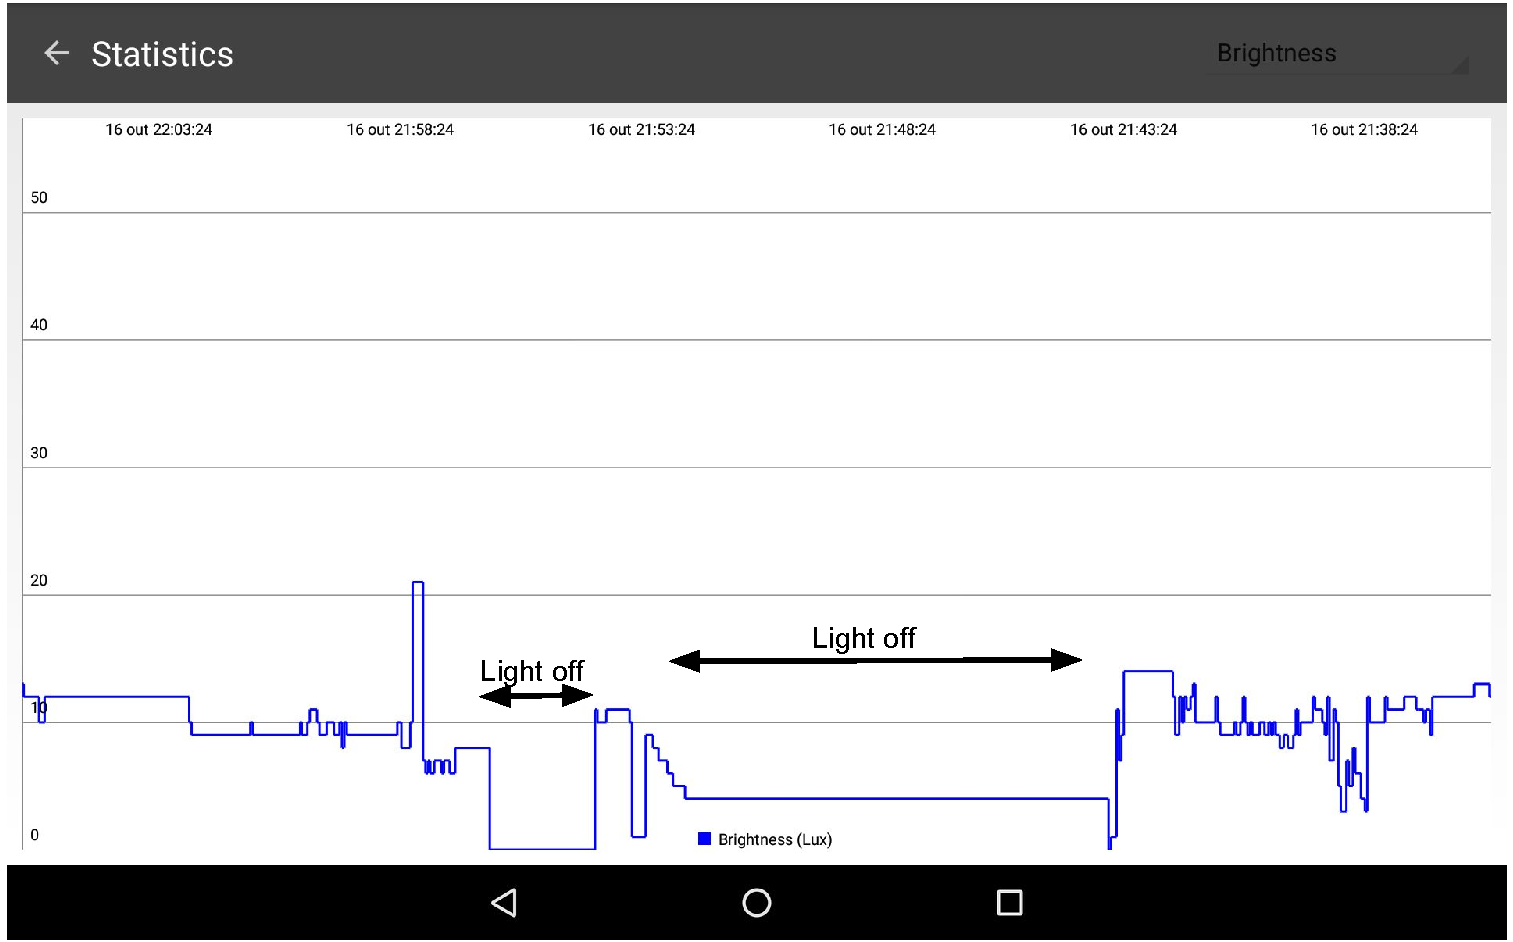
\includegraphics[width=0.45\textwidth]{Figures/eval_lights}
\caption{Luminosity Readings}
\label{eval:lights}
\end{figure}

\begin{figure}[]
\centering
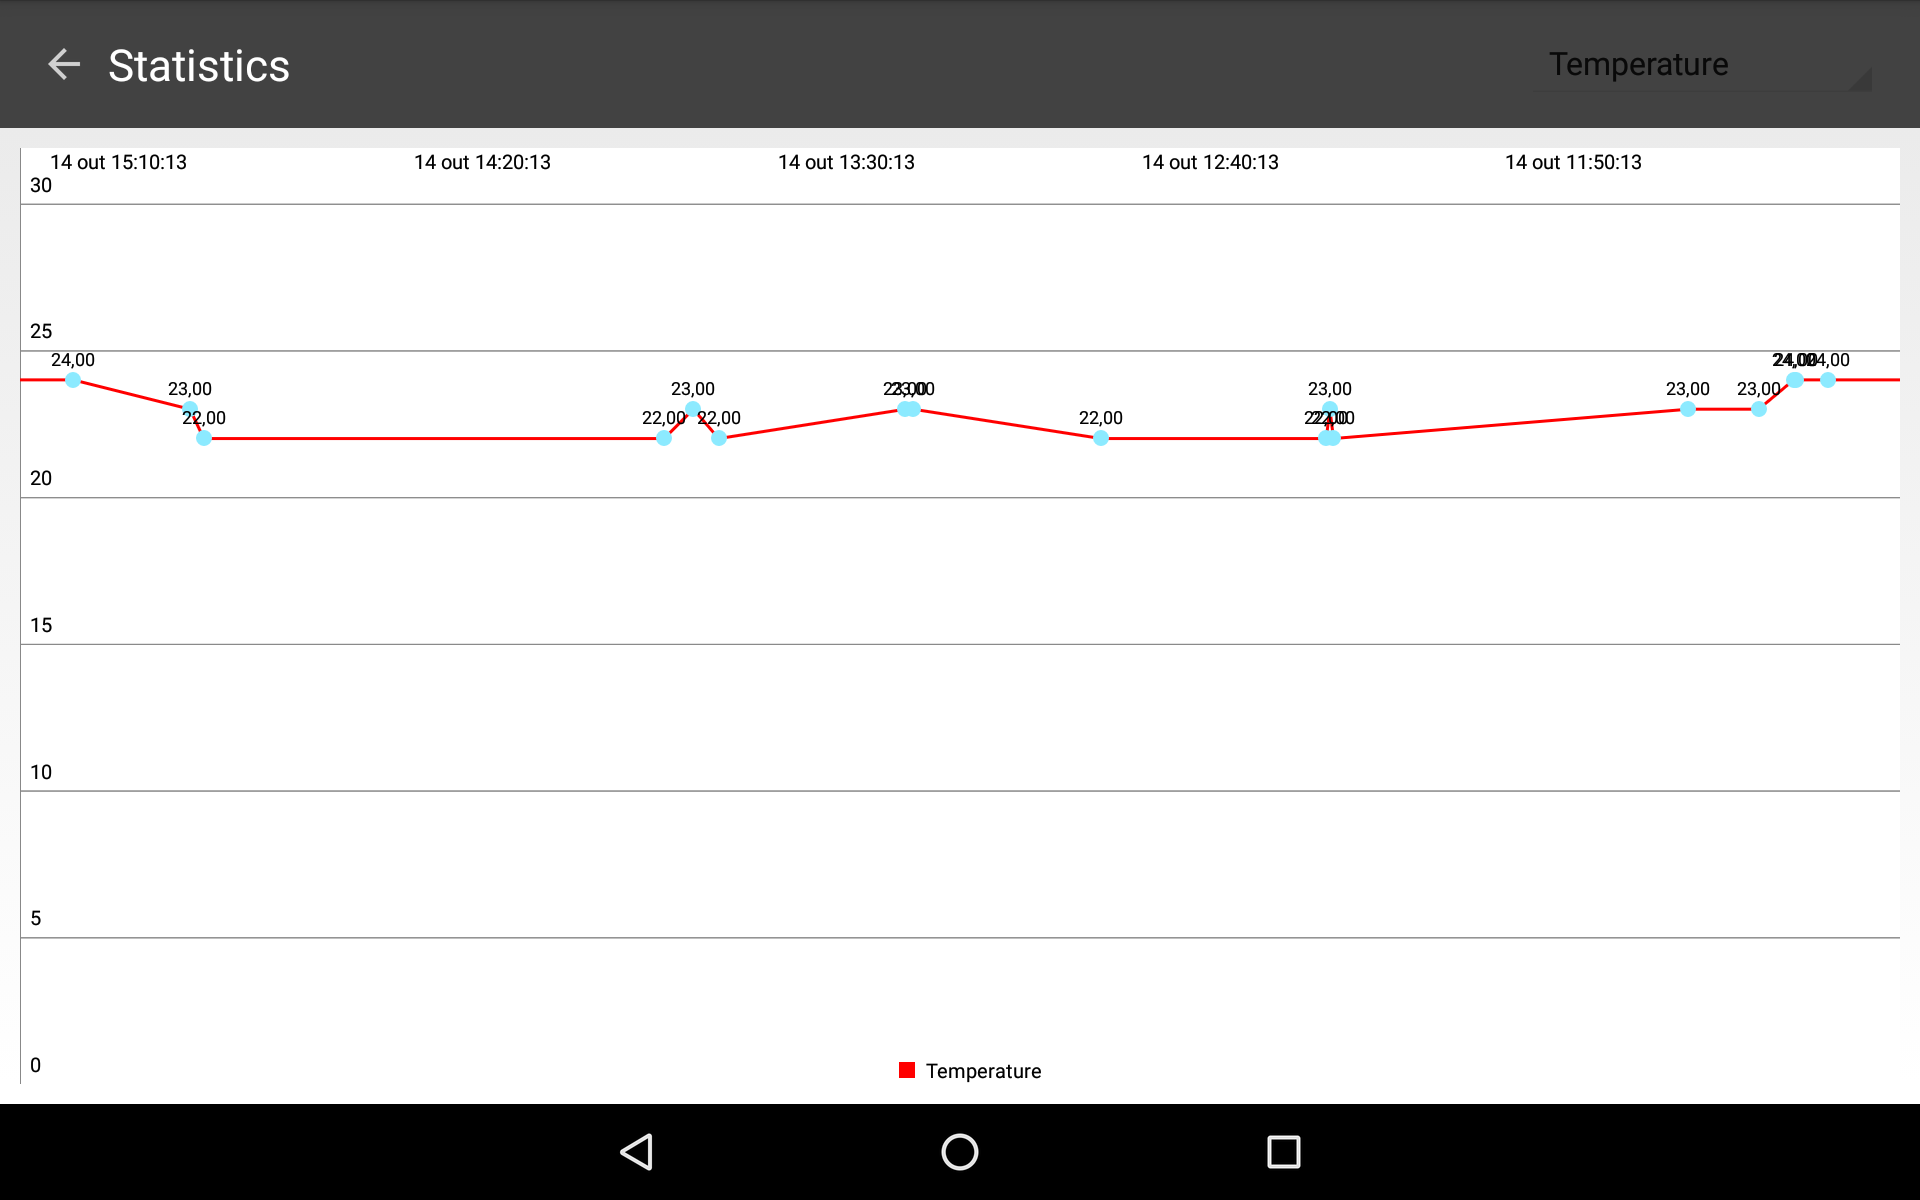
\includegraphics[width=0.45\textwidth]{Figures/eval_temp}
\caption{Temperature Readings}
\label{eval:temp}
\end{figure}

\textbf{Automation}: To evaluate the usability of the \ac{IFTTT} interface (automation recipes), user usability tests were performed with a total of 20 users. The users who performed the tests were not familiar with our system and had no previous experience with similar \ac{IFTTT} solutions.

The users were asked to create two distinct recipes:

\begin{itemize}
  \item If the user left the office, then turn off all the lights.
  \item If the temperature is above 25 ºC, then set temperature to below 20 ºC. 
\end{itemize} 

The test results were then compared to an expert user to determine the usability of the system. Comparing the results presented in Table~\ref{eval:automation2} and Table~\ref{eval:automation3} we observe that an inexperienced user took on average 19 seconds more to complete the first task in comparison with the experienced user. On average the inexperienced user took more 9 seconds to complete the second task. These values are to be expected, as first time users always under perform expert users. The extra time the first time users took is reasonable. We conclude there were no major problems in the \ac{UI} used to complete the tasks.

\begin{table}[h]
\centering
\begin{tabular}{l|r|r|}
\cline{2-3}
 & \multicolumn{1}{l|}{Task 1} & \multicolumn{1}{l|}{Task 2} \\ \hline
\multicolumn{1}{|l|}{Mean} & 36 & 27.8 \\ \hline
\multicolumn{1}{|l|}{Standard deviation} & 9.31 & 5.96 \\ \hline
\end{tabular}
\caption{User usability tests, mean and standard deviation}
\label{eval:automation2}
\end{table}


\begin{table}[h]
\centering
\begin{tabular}{l|r|r|}
\cline{2-3}
 & \multicolumn{1}{l|}{Task 1} & \multicolumn{1}{l|}{Task 2} \\ \hline
\multicolumn{1}{|l|}{Mean} & 17 & 18.4 \\ \hline
\multicolumn{1}{|l|}{Standard deviation} & 0.89 & 1.49 \\ \hline
\end{tabular}
\caption{Expert user usability tests, mean and standard deviation}
\label{eval:automation3}
\end{table}



\section*{Conclusion}

In this document, we present BASA a system that uses regular Android tablet devices running an Android application to create a \ac{BAS}. Our system aims to improve the comfort of office users, minimize wasted energy consumption of the building and provide office security monitoring. 
This is achieved by using a tablet (Hub) mounted in a wall in the office acting as a \ac{BAS}, as well as, other devices to control the lights and \ac{HVAC} system. 
We added an \ac{IFTTT} functionality that allows regular users to personalize their office automation to improve comfort and reduce wasted energy. We mitigate some problems related to user neglect by detecting the user presence in the room or building. This allows the \ac{IFTTT} automation component of our system to take certain actions based on the room and building occupancy, for example turning off the lights when no user is present inside the room.

The results presented in this thesis provide a strong foundation for future work in \ac{BAS} leveraging Android devices. 
One aspect this thesis did not focus and is pertinent to its future is the ability to connect multiple Hub instances (rooms) and take coordinated actions to improve energy efficiency and user comfort across entire sections of a building. 

Another future improvement to the system is the ability for the tablet itself to act as a \ac{BLE} beacon. This means we can use the Android device running the Hub app to achieve room level user detection and can skip the external beacon device.

During the development of our prototype, we were unable to install the Edup light switch in the wall due to a missing neutral wire. A neutral wire will have to be wired into the wall in order to deploy the prototype as originally intended. 

One aspect of our system we were not completely happy with was the user detection time in a room. The detection time should have been much lower. Further research and testing must be done to determine if it is the Android system who is not receiving the BLE signals due to energy saving policies or if it is the library by Estimote that we used that is not operating as it should.


\bibliographystyle{IEEEtran}

\addcontentsline{toc}{section}{References}
\bibliography{ref2}

% \begin{thebibliography}{1}
%
%
% \bibitem {cantrell1}
% W. H. Cantrell, ``Tuning analysis for the high-Q class-E power
% amplifier,'' \emph{IEEE Trans. Microwave Theory \& Tech.}, vol. 48,
% no. 12, pp. 2397-2402, December 2000.
% %
%
% \end{thebibliography}

\begin{acronym}
\acro{ab}{ApacheBench}
\acro{API}{application programming interface}
\acro{AP}{Access Point}
\acro{BAS}{Building Automation Systems}
\acro{BLE}{Bluetooth Low Energy}
\acro{BSS}{Basic Service Set}
\acro{BT}{Bluetooth}
\acro{CPU}{Central processing unit}
\acro{DQPSK}{Differential Quadrature Phase Shift Keying}
\acro{FFD}{full-function device}
\acro{GFSK}{Gaussian Frequency Shift Keying}
\acro{GUI}{graphical user interface}
\acro{HTTP}{Hypertext Transfer Protocol}
\acro{HVAC}{Heating, ventilation and air conditioning}
\acro{IEEE}{Institute of Electrical and Electronics Engineers}
\acro{IFTTT}{If This Then That}
\acro{IP}{Internet Protocol}
\acro{ISM}{Scientific and Medical}
\acro{IST}{Instituto Superior Técnico}
\acro{JSON}{JavaScript Object Notation}
\acro{LAN}{Local Area Network}
\acro{LR-WPAN}{low-rate wireless personal area network}
\acro{MAC}{media access control}
\acro{MS/TP}{Master-Slave/Token-Passing}
\acro{P2P}{Peer-to-peer}
\acro{PHY}{Physical Layer}
\acro{PTP}{Point-to-Point}
\acro{PerOMAS}{Personal Office Management and Automation System}
\acro{RAM}{Random-access memory}
\acro{REST}{representational state transfer}
\acro{RFD}{reduced-function device}
\acro{ROI}{Return on investment}
\acro{SAC}{access control system}
\acro{SSDP}{Simple Service Discovery Protocol}
\acro{TCP}{Transmission Control Protocol}
\acro{UDP}{User Datagram Protocol}
\acro{UI}{User Interface}
\acro{WLAN}{wireless local area network}
\acro{WPAN}{wireless personal area network}
\acro{WiFi}{Wireless fidelity}
\end{acronym}

\end{document}
